%!TEX root = ../../report.tex
\clearpage
\subsection{Process View}
\label{subsec:view-process}

\copied{Process view : The process view deals with the dynamic aspects of the system, explains the system processes and how they communicate, and focuses on the runtime behavior of the system. The process view addresses concurrency, distribution, integrators, performance, and scalability, etc. UML Diagrams to represent process view include the Activity diagram.}
{from wikipedia}
This view mainly discuss about runtime, concurrency, communication, and synchronization of the process running in the system. \\

The program flow and business logic of the system are captured in this section with the aid of activity and sequence diagrams.

\subsubsection*{Flood monitoring}
\label{subsubsec:proc-floodmonitor}

Figure~\ref{fig:activity-controlpanel} shows the activity diagram related to the control panel. As can be seen in this figure, the maintainer can login and view the faulty sensors and the issued warnings.

\begin{figure}[H]
	\centering
	\includegraphics[keepaspectratio=true,width=0.55\textwidth]{{\viewimages/control-panel}.png}
	\caption{An activity diagram of the control panel}
	\label{fig:activity-controlpanel}
\end{figure}

The activity diagram in Figure~\ref{fig:activity-monitoring} shows the flow of the flood monitoring process. The boxes represent different parts of the system. The black dots with and without a thin black circle around them represent the begin and end of a process respectively.
First of all there is the Sensor box. This box represents the activity in the sensor. It periodically reads the sensor value. After this the Arduino box gets the sensor data and sends it to the failure detection part. Here the decision is made whether the sensor data is valid or not. If it is not, the sensor will be stored in a list with faulty sensors so the maintainer can fix these sensors. Otherwise the sensor data will be normalized and stored in the database. Next the Monitoring and Flood Detection part calculates the flood probability. The probability value is also stored in the database. If the probability for a flood is high and there is an imminent flood, external data is used to create a warning. Here the warning is issued to the safety region and to the citizens through the SMS Service.

% \begin{landscape}
% 	\begin{figure}[H]
% 		\centering
% 		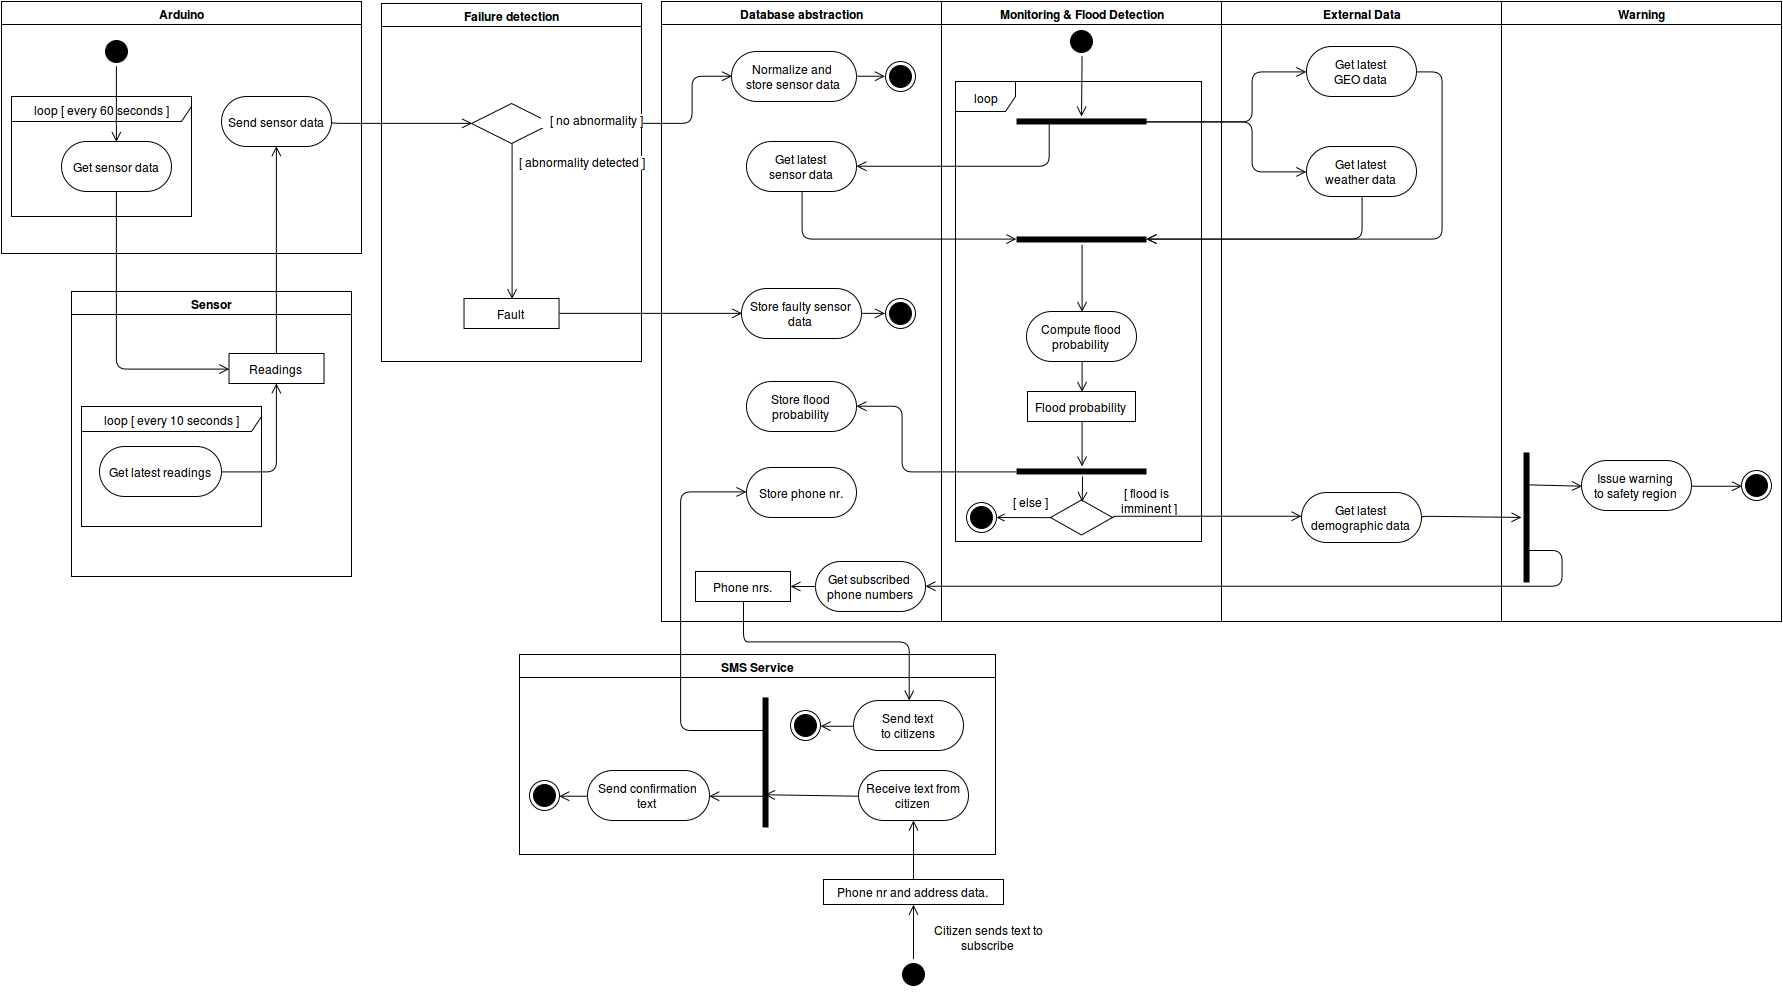
\includegraphics[keepaspectratio=true,width=1.0\textwidth]{{\viewimages/activity_monitoring}.png}
% 		\caption{An activity diagram of the flood monitoring process}
% 		\label{fig:activity-monitoring}
% 	\end{figure}
% \end{landscape}